\documentclass[10pt,a4paper,sans]{article}

\usepackage[utf8]{inputenc}
\usepackage{geometry}
\usepackage{helvet}
\usepackage[french]{babel}
\usepackage{graphicx}
\usepackage{xcolor}
\usepackage{cmlgc}

\usepackage{titlesec}
\usepackage{enumitem}
\usepackage{pifont}

\usepackage[framemethod=tikz]{mdframed}
\usetikzlibrary{shadows}

\geometry{a4paper, top=0.75cm, left=0.75cm, right=0.75cm, bottom=.75cm}

% Redéfinition format des titres/sections...
\definecolor{lightBlue}{RGB}{84, 141, 212}
\titleformat{\section}[hang]
    {\Large\color{lightBlue}\bfseries}
    {}
    {0em}
    {}[\titlerule]
\titlespacing{\section}{0cm}{0cm}{0.25cm}

\titleformat{\subsection}[hang]
        {\bfseries}
        {}
        {0em}
        {}[]
\titlespacing{\subsection}{0.25cm}{0.25cm}{0.25cm}

\titlespacing{\paragraph}{0.25cm}{0.12cm}{0.12cm}


%% Redéfinition format des listes
\setitemize[0]{label=\ding{226}, leftmargin=0.9cm, itemsep=0.12cm}

% Création des formats de cadres
\definecolor{veryLightGray}{RGB}{238, 238, 238}
\mdfdefinestyle{titre1}{backgroundcolor=veryLightGray, linewidth=0}
\mdfdefinestyle{cadreCompetences}{backgroundcolor=veryLightGray, shadow=true, shadowcolor=black, 
          linewidth=0pt, linecolor=red, shadowsize=6.5pt, leftmargin=-5pt, rightmargin=0pt, innerrightmargin=5pt}

\begin{document}

\hyphenrules{nohyphenation}

\begin{minipage}{0.36\textwidth}
    \vspace{0.30cm}
    \input{contact}
\end{minipage}
\begin{minipage}{0.62\textwidth}
    \begin{mdframed}[style=titre1]
        \begin{flushright}
            %\Large{\textbf{Ingénieur Mécanique}}
            \LARGE{\textsc{Mechanical Engineer}}

        \end{flushright}
    \end{mdframed}
    \begin{minipage}{0.75\textwidth}
        \subsection{\large{Profil :}}
        \begin{itemize}
            \item{\textbf{Flexible} capacity to learn quickly}
            \item{\textbf{Mobile} possibility of international business trip}
            \item{\textbf{Motivated} great involvement in projects}
        \end{itemize}
    \end{minipage}
    \begin{minipage}{0.23\textwidth}
        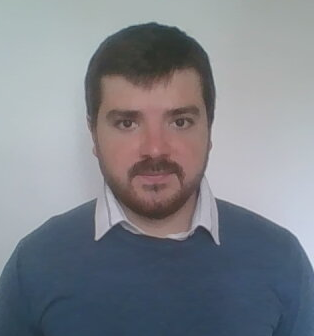
\includegraphics[width=\textwidth]{img/image_CV.png}
    \end{minipage}
\end{minipage}


\begin{minipage}[t]{0.28\textwidth}
    \begin{mdframed}[style=cadreCompetences]
        \section{Softwares}
        \subsection{Drawings}
        \begin{itemize}
            \item{Solidworks
                    \hfill
                    
\includegraphics[scale=0.25]{img/star.png} \hspace{-0.22cm}
                    
\includegraphics[scale=0.25]{img/star.png} \hspace{-0.22cm}
                    
\includegraphics[scale=0.25]{img/star.png} \hspace{-0.22cm}
                    
\includegraphics[scale=0.25]{img/star.png} \hspace{-0.22cm}
                    
\includegraphics[scale=0.25]{img/half_star.png}}
            \item{UG NX
                    \hfill
                    
\includegraphics[scale=0.25]{img/star.png} \hspace{-0.22cm}
                    
\includegraphics[scale=0.25]{img/star.png} \hspace{-0.22cm}
                    
\includegraphics[scale=0.25]{img/star.png} \hspace{-0.22cm}
                    
\includegraphics[scale=0.25]{img/star.png} \hspace{-0.22cm}
                    
\includegraphics[scale=0.25]{img/empty_star.png}}
            \item{Autocad
                    \hfill
                    
\includegraphics[scale=0.25]{img/star.png} \hspace{-0.22cm}
                    
\includegraphics[scale=0.25]{img/star.png} \hspace{-0.22cm}
                    
\includegraphics[scale=0.25]{img/star.png} \hspace{-0.22cm}
                    
\includegraphics[scale=0.25]{img/star.png} \hspace{-0.22cm}
                    
\includegraphics[scale=0.25]{img/empty_star.png}}
            \item{Creo/Pro E
                    \hfill
                    
\includegraphics[scale=0.25]{img/star.png} \hspace{-0.22cm}
                    
\includegraphics[scale=0.25]{img/star.png} \hspace{-0.22cm}
                    
\includegraphics[scale=0.25]{img/star.png} \hspace{-0.22cm}
                    
\includegraphics[scale=0.25]{img/empty_star.png} \hspace{-0.22cm}
                    
\includegraphics[scale=0.25]{img/empty_star.png}}
        \end{itemize}

        \subsection{Calculation (FEA)}
            \begin{itemize}
                \item{Solidworks
                    \hfill
                    
\includegraphics[scale=0.25]{img/star.png} \hspace{-0.22cm}
                    
\includegraphics[scale=0.25]{img/star.png} \hspace{-0.22cm}
                    
\includegraphics[scale=0.25]{img/star.png} \hspace{-0.22cm}
                    
\includegraphics[scale=0.25]{img/star.png} \hspace{-0.22cm}
                    
\includegraphics[scale=0.25]{img/empty_star.png}}
                \item{UG NX
                    \hfill
                    
\includegraphics[scale=0.25]{img/star.png} \hspace{-0.22cm}
                    
\includegraphics[scale=0.25]{img/star.png} \hspace{-0.22cm}
                    
\includegraphics[scale=0.25]{img/star.png} \hspace{-0.22cm}
                    
\includegraphics[scale=0.25]{img/star.png} \hspace{-0.22cm}
                    
\includegraphics[scale=0.25]{img/empty_star.png}}
                \item{Matlab
                    \hfill
                    
\includegraphics[scale=0.25]{img/star.png} \hspace{-0.22cm}
                    
\includegraphics[scale=0.25]{img/star.png} \hspace{-0.22cm}
                    
\includegraphics[scale=0.25]{img/star.png} \hspace{-0.22cm}
                    
\includegraphics[scale=0.25]{img/half_star.png} \hspace{-0.22cm}
                    
\includegraphics[scale=0.25]{img/empty_star.png}}
            \end{itemize}
        \subsection{Office}
            \begin{itemize}
                \item{Excel
                    \hfill
                    
\includegraphics[scale=0.25]{img/star.png} \hspace{-0.22cm}
                    
\includegraphics[scale=0.25]{img/star.png} \hspace{-0.22cm}
                    
\includegraphics[scale=0.25]{img/star.png} \hspace{-0.22cm}
                    
\includegraphics[scale=0.25]{img/star.png} \hspace{-0.22cm}
                    
\includegraphics[scale=0.25]{img/half_star.png}}
                \item{MS office
                    \hfill
                    
\includegraphics[scale=0.25]{img/star.png} \hspace{-0.22cm}
                    
\includegraphics[scale=0.25]{img/star.png} \hspace{-0.22cm}
                    
\includegraphics[scale=0.25]{img/star.png} \hspace{-0.22cm}
                    
\includegraphics[scale=0.25]{img/star.png} \hspace{-0.22cm}
                    
\includegraphics[scale=0.25]{img/empty_star.png}}
                \item{LaTex
                    \hfill
                    
\includegraphics[scale=0.25]{img/star.png} \hspace{-0.22cm}
                    
\includegraphics[scale=0.25]{img/star.png} \hspace{-0.22cm}
                    
\includegraphics[scale=0.25]{img/star.png} \hspace{-0.22cm}
                    
\includegraphics[scale=0.25]{img/half_star.png} \hspace{-0.22cm}
                    \includegraphics[scale=0.25]{img/empty_star.png}}
            \end{itemize}

        \section{Programming}
        \subsection{Applications}
            \begin{itemize}
                \item{VBA
                    \hfill
                    \includegraphics[scale=0.25]{img/star.png} \hspace{-0.22cm}
                    \includegraphics[scale=0.25]{img/star.png} \hspace{-0.22cm}
                    \includegraphics[scale=0.25]{img/star.png} \hspace{-0.22cm}
                    \includegraphics[scale=0.25]{img/star.png} \hspace{-0.22cm}
                    \includegraphics[scale=0.25]{img/star.png}}
                \item{Solidworks
                    \hfill
                    \includegraphics[scale=0.25]{img/star.png} \hspace{-0.22cm}
                    \includegraphics[scale=0.25]{img/star.png} \hspace{-0.22cm}
                    \includegraphics[scale=0.25]{img/star.png} \hspace{-0.22cm}
                    \includegraphics[scale=0.25]{img/star.png} \hspace{-0.22cm}
                    \includegraphics[scale=0.25]{img/empty_star.png}}
                \item{C
                    \hfill
                    \includegraphics[scale=0.25]{img/star.png} \hspace{-0.22cm}
                    \includegraphics[scale=0.25]{img/star.png} \hspace{-0.22cm}
                    \includegraphics[scale=0.25]{img/star.png} \hspace{-0.22cm}
                    \includegraphics[scale=0.25]{img/half_star.png} \hspace{-0.22cm}
                    \includegraphics[scale=0.25]{img/empty_star.png}}
            \end{itemize}
        \subsection{Web Developpment}
            \begin{itemize}
                \item{HTML/CSS
                    \hfill
                    \includegraphics[scale=0.25]{img/star.png} \hspace{-0.22cm}
                    \includegraphics[scale=0.25]{img/star.png} \hspace{-0.22cm}
                    \includegraphics[scale=0.25]{img/half_star.png} \hspace{-0.22cm}
                    \includegraphics[scale=0.25]{img/empty_star.png} \hspace{-0.22cm}
                    \includegraphics[scale=0.25]{img/empty_star.png}}
                \item{PHP
                    \hfill
                    \includegraphics[scale=0.25]{img/star.png} \hspace{-0.22cm}
                    \includegraphics[scale=0.25]{img/star.png} \hspace{-0.22cm}
                    \includegraphics[scale=0.25]{img/half_star.png} \hspace{-0.22cm}
                    \includegraphics[scale=0.25]{img/empty_star.png} \hspace{-0.22cm}
                    \includegraphics[scale=0.25]{img/empty_star.png}}
            \end{itemize}

        \section{Languages}
        \subsection{English : C1 \newline (855 - Toeic 2015)}
            \begin{itemize}
                \item{Understanding
                    \hfill
                    \includegraphics[scale=0.25]{img/star.png} \hspace{-0.22cm}
                    \includegraphics[scale=0.25]{img/star.png} \hspace{-0.22cm}
                    \includegraphics[scale=0.25]{img/star.png} \hspace{-0.22cm}
                    \includegraphics[scale=0.25]{img/star.png} \hspace{-0.22cm}
                    \includegraphics[scale=0.25]{img/half_star.png}}
                \item{Exrpession
                    \hfill
                    \includegraphics[scale=0.25]{img/star.png} \hspace{-0.22cm}
                    \includegraphics[scale=0.25]{img/star.png} \hspace{-0.22cm}
                    \includegraphics[scale=0.25]{img/star.png} \hspace{-0.22cm}
                    \includegraphics[scale=0.25]{img/half_star.png} \hspace{-0.22cm}
                    \includegraphics[scale=0.25]{img/empty_star.png}}
            \end{itemize}
        \subsection{German : C1 \newline (881 - WIDAF 2015)}
            \begin{itemize}
                \item{Understanding
                    \hfill
                    \includegraphics[scale=0.25]{img/star.png} \hspace{-0.22cm}
                    \includegraphics[scale=0.25]{img/star.png} \hspace{-0.22cm}
                    \includegraphics[scale=0.25]{img/star.png} \hspace{-0.22cm}
                    \includegraphics[scale=0.25]{img/half_star.png} \hspace{-0.22cm}
                    \includegraphics[scale=0.25]{img/empty_star.png}}
                \item{Exrpession
                    \hfill
                    \includegraphics[scale=0.25]{img/star.png} \hspace{-0.22cm}
                    \includegraphics[scale=0.25]{img/star.png} \hspace{-0.22cm}
                    \includegraphics[scale=0.25]{img/star.png} \hspace{-0.22cm}
                    \includegraphics[scale=0.25]{img/empty_star.png} \hspace{-0.22cm}
                    \includegraphics[scale=0.25]{img/empty_star.png}}
            \end{itemize}

        \section{Spare time}
            \begin{itemize}
                \item{squash, biketouring}
                \item{tv series, book}
                \item{robotics, web development}
            \end{itemize}
    \end{mdframed}
\end{minipage}
\hfill
\begin{minipage}[t]{0.68\textwidth}
    \vspace{0.15cm}
    \section{Training}
        \begin{itemize}
            \item{2012--2016 : \textbf{Master's degree in Mechanical Engineering} at INSA Strasbourg}
            \item{2010--2012 : German prep courses at INSA Strasbourg \textbf{DeutschInsa} \newline (half of the courses in German)}
            \item{June 2010 : Baccalauréat }
        \end{itemize}

    \section{Milton Roy : one company, several experiences}
    \subsection{June 2018 -- today : Link between Engineering department and Manager}
    \begin{itemize}%
        \item{Shared worklocation between Samoreau (Engineering department) and PSP (Production)}
        \item{Mastery of Unigraphics NX by self-training}
        \item{Mixer design : detail drawings, outline drawings and ERP data management}
        \item{Business trip to India to define mechanical calculations in MrMix} 
        \item{Training of India team to development of local market}
    \end{itemize}

    \subsection{June 2017 -- June 2018 : Mechanical engineer - dosing pump}
    \begin{itemize}
        \item{Mastery of Solidworks by self-training}
        \item{Pump design : detail drawings, outline drawings and ERP data management}
        \item{Calculation : thermal exchange, stress (FEA and analytics), natural frequency(FEA)}
        \item{Automation of outline drawings of standard dosing pumps}
    \end{itemize}

    \subsection{September 2016 -- June 2017 : Involvement in Manufacture tranfert from Samoreau to PSP}
    \begin{itemize}
        \item{Design of tank and hydraulic network to test side and top entry mixers}
        \item{Developpment of tools to analyse data of the ERP for several department (supply chain, Engineering, manufacturing,...)}
        \item{Technical support for processes adaptation and data transfer in the JD Edwards}
        \item{Development of an Excel spreadsheet to automate standard side entry BOM and drawings}
    \end{itemize}


    \subsection{2011 -- 2016 : Internship in several entities}
    \begin{itemize}
        \item{March to August 2016 -- Pont-Saint-Pierre (27) -- Rationalisation of a dosing head range.}
        \item{June to August 2015 -- Sunderland (Angleterre) -- Design of an test enclosure for high pressure equipment.}
        \item{March to August 2014 -- Samoreau (77) -- Creation of calculation spreadsheet to mixer calculations.}
        \item{June à August 2011 -- Samoreau (77) -- Measurment of propeller hydraulic properties.}
    \end{itemize}
\end{minipage}

\end{document}
